\section{Results}
\label{sec:results}

Eleven pre-registered experiments were run against the system's own codebase, each independently
verified against its own raw output. Eight reached their strongest pre-registered success
criterion; three (the dual-layer behavioral trace, the vision leakage audit, and the PSI
drift-binning sweep) reached only their pre-registered minimum-viable criterion, because each of
them found a genuine complication rather than a clean confirmation. Table~\ref{tab:goal-summary}
gives the full scorecard before the narrative below. None of the three minimum-viable results is
written around here as a shortfall -- they are, in order, the paper's central finding, a real and
now-quantified data-integrity correction, and a mechanistically explained reversal of a naive
expectation.

\begin{table}[t]
\centering
\small
\caption{Per-goal achievement summary against each goal's own pre-registered strong/minimum-viable
criteria. No goal reached \texttt{partially\_achieved}, \texttt{not\_achieved}, or \texttt{blocked}.
Source: \texttt{formalized\_results.json}.}
\label{tab:goal-summary}
\begin{tabular}{@{}lllp{7.6cm}@{}}
\toprule
Goal & Experiment & Verdict & Headline finding \\
\midrule
G1 & EXP01 & strong & RAG threshold: precision-favoring, argmax reproduced, random-baseline margin \\
G2 & EXP02 & strong & eval.py/runtime rule path is the identical module object (8/8) \\
G3 & EXP03 & minimum-viable & fail-safe defaulting dominates (50\%); fabrication survives agreement \\
G4 & EXP04 & strong & agentic tool-routing negative result, replicated at $n{=}9$ \\
G5 & EXP05 & minimum-viable & 32 near-duplicate frame pairs; corrected metric range now quantified \\
G6 & EXP06 & strong & export-format loss mechanism; INT8 loses less than fp32 \\
G7 & EXP07 & strong & configured-threshold recall (0.782) $\ne$ headline argmax recall (0.719) \\
G8 & EXP08 & minimum-viable & PSI binning sensitivity crossover, not confirmed monotonic \\
G9 & EXP09 & strong & twin\_bridge: unit-tested, never live-validated \\
G10 & EXP10 & strong & no closer prior instance of the cross-layer thesis found \\
G11 & EXP11 & strong & manuscript-wide audit; found a live, unfixed stale figure \\
\bottomrule
\end{tabular}
\end{table}

\subsection{The dual-layer decision system: fail-safe defaulting, not correction}
\label{sec:results-dual-layer}

% SOURCE_CLAIM: experiment_workspace/experiment_runs/EXP02/results.md (8/8 module-identity check)
The claim that the evaluation harness and the system's own decision path compute severity identically was verified at
the strongest available level: both resolve to the exact same in-memory \texttt{rules} module
object (a Python \texttt{is} identity check, not output-matching), with 8/8 scenario agreement.
This closes, structurally, the specific failure mode that motivated building this check in the
first place -- a copied rule engine silently drifting from the system's real decision path.

That structural guarantee only tells us the two paths compute the \emph{same} severity given the
same inputs. It says nothing about what AQUA-1B's actual output looks like, or how often the
escalation it is supposed to trigger actually fires. Recall that every result in this subsection
was obtained against the configured \texttt{sure-aqua-adapter}, trained on eight handwritten examples
that the project's own fine-tuning script documents as insufficient, smoke-test-only material --
not the properly sized, 128-example alternative that sat unused on disk before this adapter was
even trained (Section~\ref{sec:dual-layer}). That is stated here again, deliberately, because it is
the fact that changes how the following result should be read.

% SOURCE_CLAIM: experiment_workspace/experiment_runs/EXP03/results.md (4-bucket table, n=8);
% experiment_workspace/experiment_runs/EXP03/g3_results.json (per-scenario raw outputs)
One might expect a dual-layer safety system's value to come from the rule engine catching the
model's occasional wrong call. It rarely gets the chance to: half the time (4/8) the model's
output does not parse at all, and -- more surprising still -- even when its final status agreed
with the rule engine, in two of those three cases the reasoning behind it cited a sensor value
that was never in the input. Figure~\ref{fig:exp03-buckets} shows the full four-bucket
distribution across all 8 of the evaluation harness's scenarios ($n=8$, the entire fixed scenario
population; no confidence interval is implied): 50\% unparseable-defaulted-to-\texttt{ok}, 38\%
parseable-and-agrees, 12\% parseable-and-under-calls-and-escalated, and 0\% parseable-and-over-calls
(too small an $n$ to conclude over-calls are rare in general -- only that none occurred here).
Manual, single-rater coding of all 8 free-text reasoning strings against each scenario's true,
synthetically generated sensor snapshot found 6 of 8 materially misrepresent that snapshot -- of
those, 3 (T02, T05, T08) fabricate a specific numeric sensor value never present in the input
(stating, for instance, dissolved oxygen 6.0~mg/L against the scripted test scenario's actual input
value of 5.7 -- itself a synthetically generated test value, not a live reading), and the remaining
3 are inaccurate in
a different way -- an unsupported blanket claim with no invented number (``all parameters
optimal'' during an active multi-parameter emergency) or an internally incoherent reading of a
plausibly real value. In two cases (both inside the ostensibly cleanest ``agrees'' bucket) the
categorically correct final status is reached via an entirely invented causal narrative built on a
fabricated number. Whenever that 38\% agrees figure is quoted anywhere in this paper, this same
fabrication rate belongs beside it: the number is not a measure of the model reasoning correctly
two-thirds of the time it agreed with the rule engine, because in two of three such cases it did
not.

\begin{figure}[t]
\centering
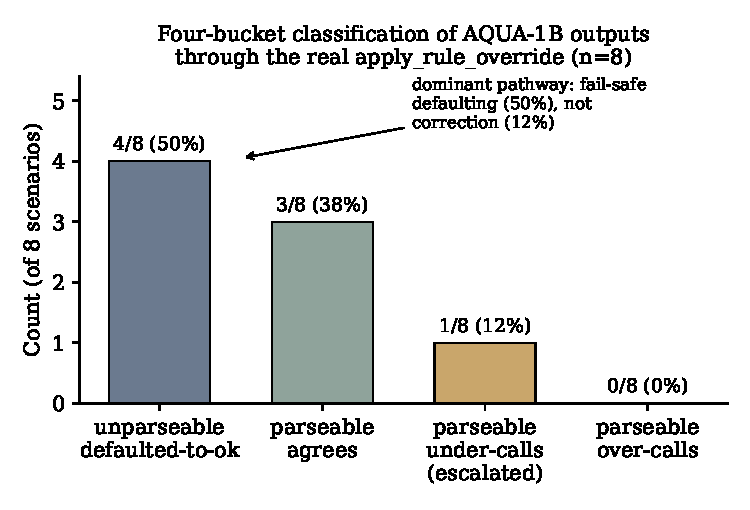
\includegraphics[width=0.62\linewidth]{figures/fig1_exp03_four_bucket.pdf}
\caption{Four-bucket behavioral classification of AQUA-1B's output against the real, unmodified
\texttt{apply\_rule\_override} path, across all 8 evaluation-harness scenarios ($n=8$, single local
1B model with an 8-example smoke-test adapter, single rater for the reasoning-content coding
pass). The dominant observed pathway is malformed-output fail-safe defaulting (50\%), not
sophisticated severity correction (12\%); zero over-calls were observed, but $n=8$ is too small to
conclude the over-call bucket is rare in general.}
\label{fig:exp03-buckets}
\end{figure}

We did not give the LLM a fair chance -- the configured adapter trained on 8 handwritten examples the
project's own training pipeline calls insufficient, while a documented, properly sized 128-example
alternative sat unused on disk -- and the architecture's safety property held anyway. Stated
without hedging, because it should not read as an apology: this makes the finding above stronger
evidence for the architecture's design, not weaker. A model given close to no fair chance to reason
well still could not push the system's final severity below what the rule engine alone would
compute in any of the 8 scenarios, including the one case (T02, a critical dissolved-oxygen
scenario) where its own proposed status was wrong. The safety property measured here never
depended on AQUA-1B reasoning correctly. It depended on one enumerable field being extractable from
whatever the model produced, and on the system defaulting to a safe state when it was not --
exactly Formalization~\ref{form:enumerable}'s boundary, now with a concrete, in-system instance
rather than a theoretical one. \texttt{backend/test\_decision.py}'s own mechanism-correctness suite
(18/18 passing under synthetic fixtures) confirms the override logic itself is implemented
correctly; it is reported here strictly apart from the behavioral finding above, because a passing
unit test says nothing about how a real model's output actually distributes across that logic's
branches.

\subsection{Agentic tool-routing: a negative result that survives an adversarial re-run}
\label{sec:results-agentic}

% SOURCE_CLAIM: experiment_workspace/experiment_runs/EXP04/results.md (aqua1b_results.jsonl,
% aqua7b_results.jsonl); base model, no LoRA adapter loaded for either model in this experiment
The adapter-provenance caveat above does not apply to this subsection: both models here ran base
weights, with no adapter loaded at all. AQUA-1B never produces a parseable tool call under the
system's closed-menu agent loop -- 0\% format compliance, 0\% tool-selection accuracy, on both the
original 5-scenario benchmark and a deliberately adversarial re-run designed to break the
result rather than confirm it. That re-run added four newly authored scenarios the model had never
seen, built specifically to test whether AQUA-1B's failure is prompt-specific: it is not. AQUA-1B's
0\%/0\% failure holds identically on all four new scenarios, for $n=9$ total.

AQUA-7B, the larger model, holds the response format more often but chooses the same tool,
\texttt{get\_sensor\_trend}, as its first action in every one of 9 genuinely independent scenarios
-- including two scenarios where that tool is not among the acceptable answers at all. This is a
constant answer, not evidence of discrimination between scenarios, and the benchmark's own
constant-answer check correctly flags it as such rather than letting the raw selection percentage
(which nominally rose from 50\% to 71.4\% on the larger scenario set, an artifact of three of the
four new scenarios happening to be sensor-trend-relevant by design) stand uncontextualized. We tried
to break this finding by growing the scenario set and it got stronger, not weaker: nine independent
samples of a model emitting the same answer regardless of scenario content is harder to explain
away as a small-sample coincidence than five. One disclosed discrepancy against the system's own
published benchmark table: format compliance and mean step count for AQUA-7B did not reproduce
exactly on this re-run (100\%/2.0 steps measured here versus a previously published 60\%/3.6),
while the selection percentage and the constant-answer conclusion reproduced exactly; no
configuration difference was found to explain the discrepancy, and it is reported as an unexplained,
non-conclusion-changing drift rather than silently reconciled.\footnote{Most likely explained by
version drift in the underlying \texttt{mlx-lm}/model-serving stack between the original benchmark
run and this reproduction; not investigated further, as it does not affect either model's negative
result.}

\subsection{Edge vision: an honest re-measurement, and a counter-intuitive export finding}
\label{sec:results-vision}

% SOURCE_CLAIM: initial_context/MODEL_RAPORU.md and vision.md (headline reported figures);
% experiment_workspace/experiment_runs/EXP06/results.md, EXP06/run1_full_table.json (fresh
% six-config reproduction)
The system's detector (YOLOv11s, trained on 510 labeled images, single class \texttt{sturgeon}) is
reported at mAP50 0.840, precision 0.858, recall 0.719.\footnote{A fresh reproduction of
\texttt{model.val()} on the exact configured checkpoint (\texttt{best.pt}, epoch 77) in this audit
returned precision 0.859 and mAP50 0.8395 -- a thousandths-place rounding difference against the
reported 0.858/0.840, not a new discrepancy; recall reproduced exactly at 0.719. Table~\ref{tab:stale-figures}, row 3, records this for completeness.} These are the numbers a
validation report headlines by convention: the confidence threshold that maximizes F1 on the
held-out curve. They are not, however, the numbers the system's configured threshold actually
produces.

Formalization~\ref{form:operatingpoint} named this distinction in the abstract; here it is
concrete. The configured confidence threshold (\texttt{CONF\_THRESH=0.20}, confirmed by direct
reading of \texttt{yolo\_runner.py}, deliberately lowered from 0.30 for recall on crowded frames)
selects a different point on the precision--recall curve than the F1-argmax. Figure~\ref{fig:exp07-pr}
plots both.

\disclosure{At the configured threshold, the detector actually runs at precision 0.720 / recall
\textbf{0.782} -- lower precision, \emph{higher} recall than the headline P=0.858/R=0.719 the rest
of this paper otherwise cites (functionally the true F1-argmax, at conf$\approx$0.341, differing
by only 0.0008 in F1). Both numbers are correct; they answer different questions. For any claim
about full-frame-miss risk under the system's configured operating point -- the quantity that feeds
the downstream \texttt{fish\_count==0} safety rule -- \textbf{0.782 is the number that governs it},
not 0.719. This
is more reassuring than a naive reading of ``recall 0.719'' suggests, not less, and it is stated
here explicitly because the manuscript-wide provenance audit (Section~\ref{sec:results-audit})
found no existing document distinguished the two numbers.}

\begin{figure}[t]
\centering
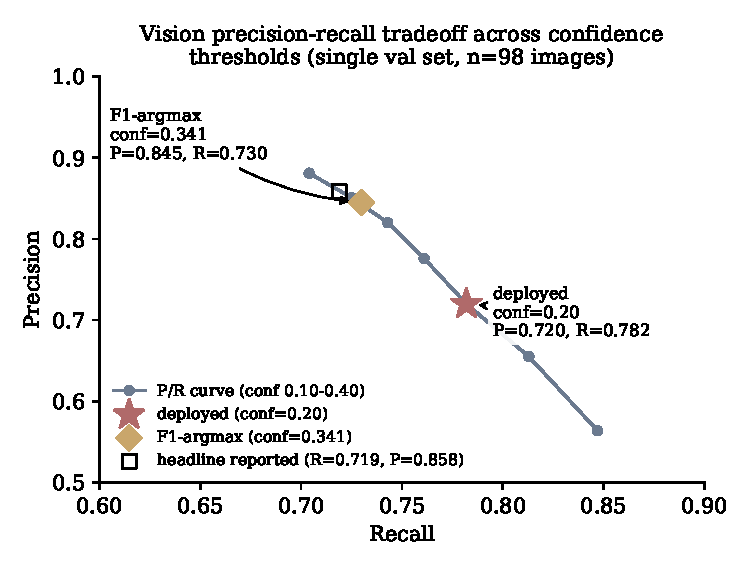
\includegraphics[width=0.62\linewidth]{figures/fig2_exp07_pr_tradeoff.pdf}
\caption{Precision--recall tradeoff across confidence thresholds (single validation set, $n=98$
images, single device). The academic-style F1-argmax is functionally identical to the headline
reported metric ($\Delta F1 = 0.0008$), but the system's configured operating point differs: the
confidence threshold trades precision for recall, actually operating at $R=0.782$.}
\label{fig:exp07-pr}
\end{figure}

% SOURCE_CLAIM: experiment_workspace/experiment_runs/EXP07/results.md,
% exp07_fish_per_frame_summary.json, exp07_per_frame_detail.json
Measured directly against all 98 validation frames, zero produced no detections at all at the
configured threshold (0/98 full-frame misses), consistent with an independence approximation that
predicted an expected 0.053 misses over the same set. This result carries a coverage gap that
belongs beside it, not in a separate limitations paragraph read later: the validation set's minimum
ground-truth fish count per frame is $k=3$; it contains \emph{zero} frames with $k=1$ or $k=2$ fish.
The full-frame-miss regime most relevant to a genuinely sparse or isolated fish -- exactly the case
a welfare check most needs to catch -- was never designed into this dataset and cannot be measured
from it. Extrapolating the same independence approximation to $k=1$ suggests a miss probability of
roughly 22--28\% depending on which recall figure is used; this is an untested extrapolation, stated
as one, not a measurement.

% SOURCE_CLAIM: experiment_workspace/experiment_runs/EXP05/results.md,
% experiment_workspace/experiment_runs/EXP05/g5_resolution_corrected_metrics_full.json
A separate audit of the train/validation split found 32 near-duplicate frame pairs at a strict
perceptual-hash threshold, 14 of them immediately adjacent frame indices of the same source video
-- a real, previously undocumented leakage risk, milder than and distinct from an already-corrected
exact-duplicate case elsewhere in this dataset's history. A same-checkpoint re-evaluation on the
validation set with the affected frames excluded (not a leakage-free retrain: the flagged training
frames remain in the set that produced this checkpoint's weights) gives a corrected range of precision
0.846--0.852, recall 0.712, mAP50 0.8335--0.8345, depending on how conservatively the exclusion is
drawn -- a real but modest 0.5--1.3 point optimistic bias, smaller than the dataset's already-known
leakage case and not conclusion-changing. Table~\ref{tab:headline-metrics} reports both the
uncorrected and corrected ranges together, and this caveat sentence should travel with the headline
vision numbers wherever they are cited outside this paper as well.

\begin{table}[t]
\centering
\small
\caption{Headline metrics across the four measured layers, with the G5-corrected vision range
shown alongside the uncorrected headline where applicable. The correction is a same-checkpoint
re-evaluation on a smaller held-out set, not a leakage-free retrain.}
\label{tab:headline-metrics}
\begin{tabular}{@{}p{5.4cm}p{3.0cm}p{3.0cm}l@{}}
\toprule
Metric & Headline & G5-corrected & Source \\
\midrule
Vision mAP50 ($n{=}98$) & 0.8395 & 0.8335--0.8345 ($n{=}81\text{-}85$) & EXP06/EXP05 \\
Vision precision & 0.858--0.859 & 0.846--0.852 & EXP06/EXP05 \\
Vision recall (F1-argmax) & 0.719 & 0.712 & EXP07/EXP05 \\
Vision recall (\emph{configured}, conf=0.20) & \textbf{0.782} & --- & EXP07 \\
Edge latency, CoreML/ANE p50/p95 & 9.03/9.60 ms & --- & EXP06 \\
RAG: MRR (e5-small/heading) vs.\ random & 0.856 vs.\ 0.418 & --- & EXP01 \\
RAG: hit@1 vs.\ random & 0.793 vs.\ 0.207 & --- & EXP01 \\
INT8 export $\Delta$mAP50 vs.\ fp32 export & $-0.0082$ vs.\ $-0.0104$ & --- & EXP06 \\
\bottomrule
\end{tabular}
\end{table}

% SOURCE_CLAIM: experiment_workspace/experiment_runs/EXP06/results.md, run1_full_table.json,
% run2_coreml_only.json, run3_coreml_only.json, g6_onnx_ts_diff_summary.json
Export-format benchmarking across six configurations of the same checkpoint
(Figure~\ref{fig:exp06-scatter}) reproduces the configured CoreML/ANE latency figure as genuinely
stable across sessions, not a single lucky sample: p50 $9.03 \pm 0.22$~ms, p95 $9.60 \pm 0.18$~ms
across three independent process invocations, nearly four to five times faster than any CPU-based
export while costing under one accuracy point relative to the fp32 baseline. One might expect the
more aggressively compressed format to pay the larger accuracy cost. INT8 quantization loses
\emph{less} ($\Delta$mAP50 $-0.0082$) than the unquantized fp32 ONNX and TorchScript exports
already do ($-0.0104$) -- the loss lives in a shared export/post-processing path, not in the
numeric precision that gets blamed by default. A new per-image diff between the ONNX and
TorchScript exports found 0 of 98 validation images meaningfully different (median matched-pair
IoU $0.99999976$), direct evidence that the two exports' shared loss is systematic rather than
independent numerical noise, though this diff shows the two exports agree with \emph{each other},
not a full isolation of which specific stage of the shared post-processing path is responsible.

\begin{figure}[t]
\centering
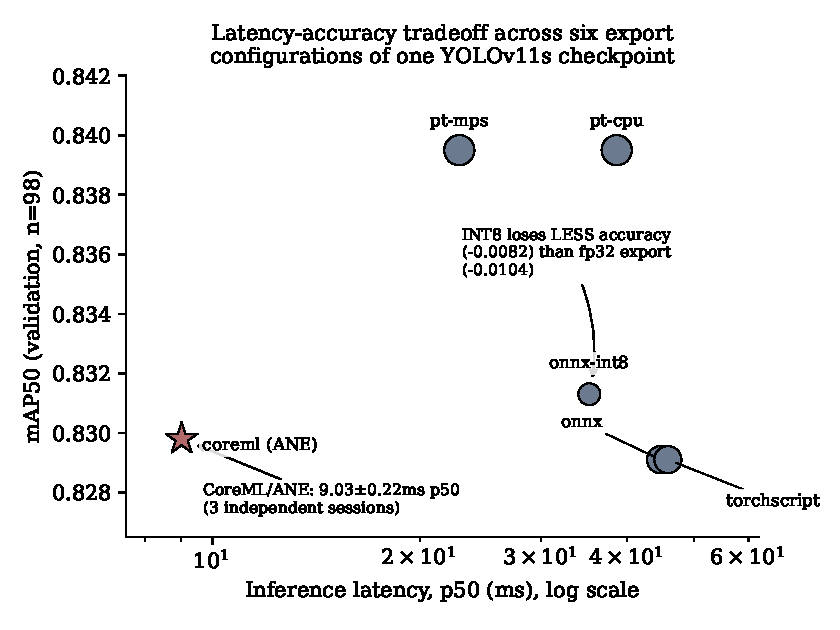
\includegraphics[width=0.68\linewidth]{figures/fig3_exp06_export_latency_map50.pdf}
\caption{Latency--accuracy tradeoff across six export configurations of the same YOLOv11s
checkpoint (single validation set, $n=98$ images, single Apple M4 Pro device; latency is
model-inference-only, not representative of network round-trip in a cloud-served alternative).
CoreML/ANE (starred) is both the fastest and within one mAP50 point of the fp32 baseline.}
\label{fig:exp06-scatter}
\end{figure}

\subsection{RAG: an asymmetric-cost threshold, not a raw F1 optimum}
\label{sec:results-rag}

% SOURCE_CLAIM: experiment_workspace/experiment_runs/EXP01/results.md,
% experiment_workspace/experiment_runs/EXP01/calibrate_output.log,
% random_baseline_results.json
The configured retrieval threshold (0.85) is one step above the empirical F1-optimum (0.84, F1 0.951
versus 0.906 at the configured threshold), trading 17.2 points of recall for zero negative-retrieval leakage
(precision 1.000 at 0.85 versus 0.906 at 0.84). Figure~\ref{fig:exp01-threshold} shows the full
sweep; the positive and negative similarity distributions genuinely overlap on this corpus
(negative max 0.847 exceeds positive min 0.841), so no threshold fully separates them, and the
model's own instruction to decline an unanswerable query is doing real, unmeasured work a
similarity cutoff cannot substitute for. This is a deliberate, disclosed asymmetric-cost choice,
not an unexamined default: a missed document only weakens reasoning the rule engine still
adjudicates independently, while a passed negative hands the model irrelevant material to blend
into a confidently cited, wrong answer. A new random-retrieval baseline (uniform selection over the
corpus's 44 chunks, stable across 5 seeds) confirms the configured retriever's measured skill is real
semantic retrieval and not a small-corpus artifact: hit@1 margin +0.586 (0.793 versus 0.207), MRR
margin +0.438 (0.856 versus 0.418) over random chance.

\begin{figure}[t]
\centering
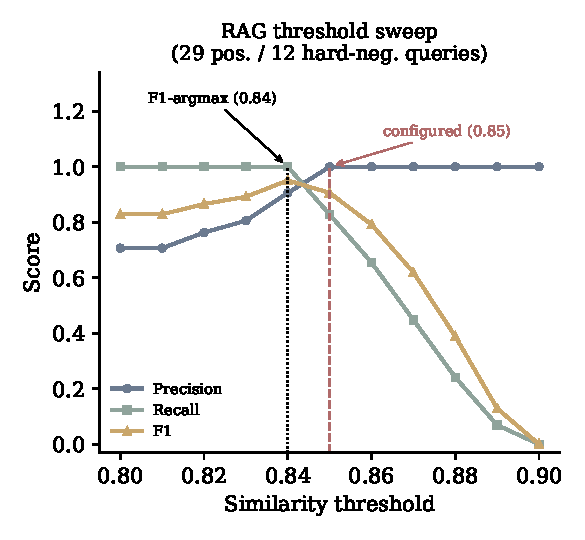
\includegraphics[width=0.5\linewidth]{figures/fig5_exp01_rag_threshold.pdf}
\caption{Precision/recall/F1 sweep over the RAG similarity threshold (single 8-document/44-chunk
corpus, 29 evaluation queries). The configured threshold (0.85) sits one step above the F1-optimum
(0.84), a deliberate precision-favoring choice.}
\label{fig:exp01-threshold}
\end{figure}

\subsection{MLOps and drift detection: a crossover, not a confirmation}
\label{sec:results-mlops}

% SOURCE_CLAIM: experiment_workspace/experiment_runs/EXP08/results.md,
% experiment_workspace/experiment_runs/EXP08/exp08_output.json (full 16-point sweep)
A 16-point severity sweep over quantile and equal-width PSI binning does not confirm the naive
expectation that equal-width binning misbehaves early and quantile binning grades smoothly
throughout. It confirms something more specific and, on inspection, more useful.
Figure~\ref{fig:exp08-psi} shows quantile binning is \emph{more} sensitive than equal-width at
small early shifts ($\delta \le 0.06$: at $\delta=0.02$, quantile PSI 0.164 already reads
``moderate'' while equal-width's 0.078 still reads ``none''), and only from $\delta \ge 0.08$
onward does equal-width overtake and grow more explosively (at $\delta=0.30$: 7.649 versus 4.844).
Per-bin decomposition traces the mechanism directly: the detector's confidence scores cluster in a
narrow band, so one large fixed equal-width bin holds roughly 30\% of the reference mass; once a
shift empties that bin, its own log-ratio term alone dominates the equal-width total. Quantile
binning, with no single bin holding more than about 10\% of reference mass by construction, has no
comparable single point of failure. The correct summary is a crossover with a mechanistic
explanation, not ``quantile binning is more sensitive, use quantile'' -- at $\delta \ge 0.08$ the
relationship reverses, and a practitioner choosing a binning scheme from this result alone would
need to know which severity regime their own drift is expected to occur in.

\begin{figure}[t]
\centering
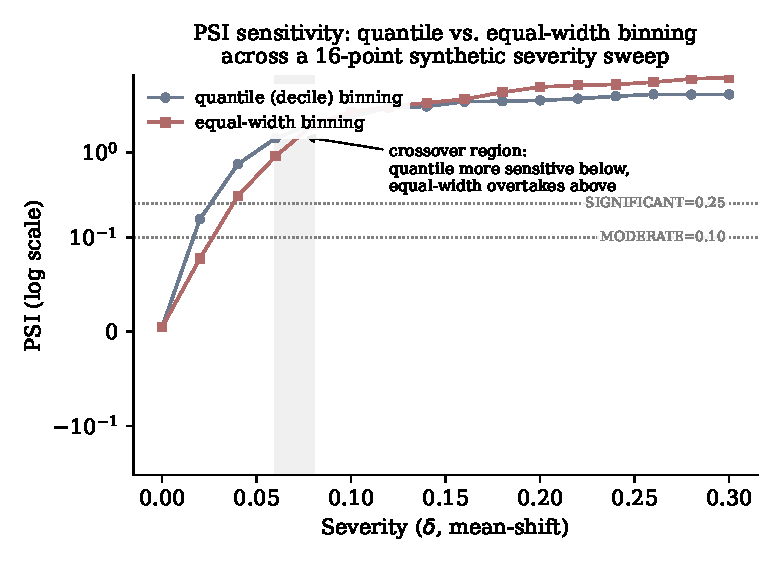
\includegraphics[width=0.68\linewidth]{figures/fig4_exp08_psi_sweep.pdf}
\caption{PSI computed via quantile (decile) versus equal-width binning across a 16-point synthetic
mean-shift severity sweep on detection-confidence scores ($n=1467$ per window). Equal-width
binning is \emph{less} sensitive than quantile at small early shifts but becomes more explosive
once a single large fixed bin empties, confirmed by per-bin decomposition.}
\label{fig:exp08-psi}
\end{figure}

The three-way retraining gate this sweep feeds was exercised directly against two synthetic
windows and behaved exactly as designed: a no-drift window (PSI 0.0048) yielded a \texttt{none}
decision, and a significant-drift window (PSI 0.9070) yielded \texttt{retrain}. The promotion gate
itself correctly rejected a candidate that failed to beat the incumbent, correctly rejected a
candidate whose improvement (+0.0025 mAP50) sat inside the fixed noise band, and correctly accepted
a candidate that cleared it (+0.015 mAP50) -- all three outcomes matching the gate's documented
behavior exactly.\footnote{One internal inconsistency, self-contained and non-conclusion-changing:
the sweep's own $\delta=0.04$ entry (quantile PSI 0.7279) differs from a separately drawn
significant-drift window at the same nominal $\delta$ (PSI 0.9070), an artifact of unseeded
per-call resampling inside an otherwise fixed-seed script. No headline number in this paper depends
on either individual value.}

\subsection{Auxiliary evidence and manuscript-wide provenance audit}
\label{sec:results-audit}

The system's third-party digital-twin comparison module, \texttt{twin\_bridge}, is designed and
unit-tested -- its existing test suite passes 18 of 19 cases (the one failure traces to a
float-truncation bug in a test helper, not the actual decoding logic it tests), and four new
edge-case tests targeting a previously unreached comparison branch all pass -- but it has never
been exercised against a live Godot or CODESYS session, and no such session exists anywhere in this
project's history. Every test in this subsystem, existing and new, is team-authored mechanism
evidence run against a scripted double, not evidence from an independently produced external
system, and it is described that way throughout this paper: unit-tested, never field-validated.

% SOURCE_CLAIM: experiment_workspace/experiment_runs/EXP11/results.md, provenance_table.json
A manuscript-wide audit re-verified every headline number in this paper against its raw source
file and git commit, and re-ran a repository-wide grep for a specific recall figure (0.695) this
project's history required guarding against, after an earlier mislabeled-checkpoint error was
corrected. That grep passes everywhere the figure could reach a reader of this paper -- but it
surfaced something outside the paper's own text: the system's RAG knowledge base itself still
states, as a live fact, that the detector's recall is ``\textasciitilde0.695,'' 43 minutes'
worth of commits behind the correction applied everywhere else, and unfixed at the time of this
audit. This is not a citation error a reader of this paper could ever encounter directly. It is a
retrievable, user-facing stale claim inside the system's own retrieval corpus -- the
exact hazard a fabrication-and-disclosure discipline paper should least want to find inside its
own codebase, and it is reported here rather than quietly fixed and never mentioned.
Table~\ref{tab:stale-figures} lists this alongside five smaller inconsistencies the same audit
found, in descending severity.

\begin{table}[t]
\centering
\small
\caption{Stale or internally inconsistent figures identified by the manuscript-wide provenance
audit (EXP11), disclosed rather than silently corrected or omitted. Row 1 is a live, unresolved
data-integrity issue in the system's own knowledge base, distinct from anything in this
manuscript's own text.}
\label{tab:stale-figures}
\begin{tabular}{@{}p{0.46\linewidth}p{0.2\linewidth}p{0.12\linewidth}p{0.12\linewidth}@{}}
\toprule
Description & Value(s) & Severity & Status \\
\midrule
Live recall figure in the RAG knowledge base & 0.695 & HIGH & not fixed \\
Recall ambiguity: F1-argmax vs.\ configured point & 0.719 vs.\ 0.782 & MEDIUM-HIGH & disclosed here \\
Precision rounding: reported vs.\ raw re-derivation & 0.858 vs.\ 0.859 & LOW & footnoted \\
AQUA-7B agent-benchmark drift: published vs.\ re-run & 60\%/3.6 vs.\ 100\%/2.0 & MEDIUM & footnoted \\
EXP08 internal PSI resampling inconsistency ($\delta$=0.04) & 0.7279 vs.\ 0.9070 & LOW & footnoted \\
Vision leakage caveat not yet propagated to headline numbers & 32 pairs, 14 adjacent & MEDIUM & resolved here (Table~\ref{tab:headline-metrics}) \\
\bottomrule
\end{tabular}
\end{table}
